% paper/sections/results.tex

\section{Results}
\label{sec:results}

\subsection{Training-Distribution Performance}
\label{sec:train_results}

All three \SAC{} conditions achieve near-perfect success (${\geq}95\%$)
on the training distribution after $10^6$ steps, confirming that each
policy learned goal-reaching under its respective physics regime.
The \PID{} controller achieves $100\%$ training success with mean reward
$-7.1$.
We therefore focus the remainder of this section on the held-out test
distribution, which represents genuinely out-of-distribution fluid
dynamics never encountered during training.

\begin{figure}[!t]
  \centering
  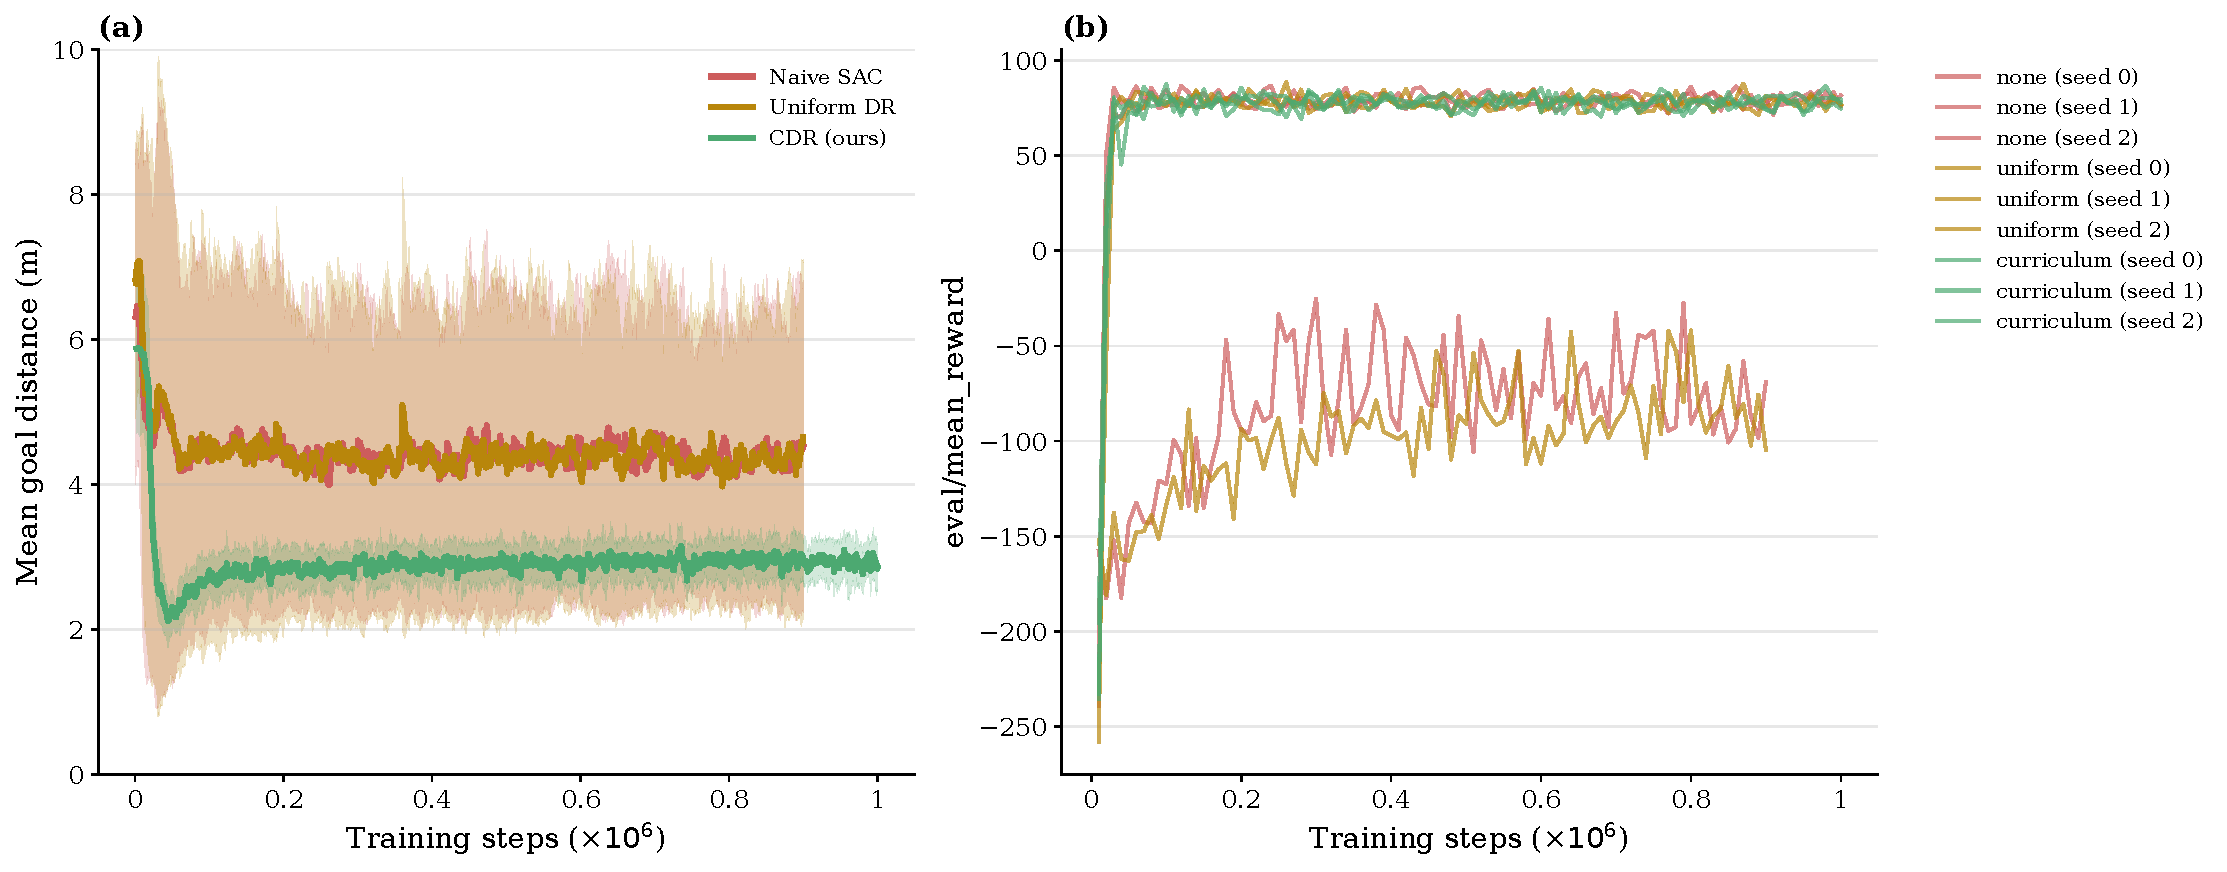
\includegraphics[width=\columnwidth]{figures/fig2_mixed_curves.pdf}
  \caption{%
    Training reward curves for all three \SAC{} conditions
    (mean~$\pm$~std across $3$~seeds, shaded). \CDR begins lower
    due to narrow initial ranges but converges within $\sim\!300$k
    steps, consistent with sequential difficulty exposure.%
  }
  \label{fig:training_curves}
\end{figure}

% ─── 5.2 ────────────────────────────────────────────────────
\subsection{PID Fragility Under Distribution Shift}
\label{sec:pid_results}

Table~\ref{tab:main_results} presents transfer evaluation results.
The \PID{} controller achieves $100\%$ success under nominal physics
yet collapses to $3.0\%$ on the held-out test distribution
(reward: $-7.1 \to -249.0$), a $97$-percentage-point drop.

This collapse arises from two interacting effects.
First, water currents at $0.40$--$0.80$\,m/s continuously displace
the \AUV{}; the proportional term cannot distinguish current-induced
error from inertia-induced error, causing runaway integral accumulation.
Second, quadratic drag at $0.60$--$1.20$\,kg/m decelerates the \AUV{}
$3$--$6{\times}$ faster than at nominal conditions; gains tuned for
nominal drag over-command thrust, inducing overshoot and limit-cycle
oscillation around the goal.
This $97$-pp collapse---to our knowledge the most precise quantification
of PID fragility under fluid-parameter shift in the AUV RL
literature---directly motivates physics-aware training.

% ─── 5.3 ────────────────────────────────────────────────────
\subsection{Domain Randomisation Eliminates Deployment Variance}
\label{sec:dr_results}

Naive \SAC{} achieves $47.67\%\,{\pm}\,33.83\%$ transfer
success across three seeds.
This $\pm 33.83$\,pp inter-seed variance represents a
\emph{deployment lottery}: the same training procedure yields policies
ranging from near-non-functional to moderately robust, with no way to
predict outcome from training curves alone.

Both \DR{} conditions eliminate this variance.
\UDR{} achieves $73.33\%\,{\pm}\,37.71\%$ and
\CDR{} achieves $98.67\%\,{\pm}\,1.89\%$, both
with near-zero inter-seed variance.
This confirms that physics-parameter coverage during training is
\emph{necessary and sufficient} for consistent transfer: the specific
scheduling strategy (uniform vs.\ curriculum) has less impact on success
rate than the presence or absence of \DR{} itself.

\begin{figure*}[!t]
  \centering
  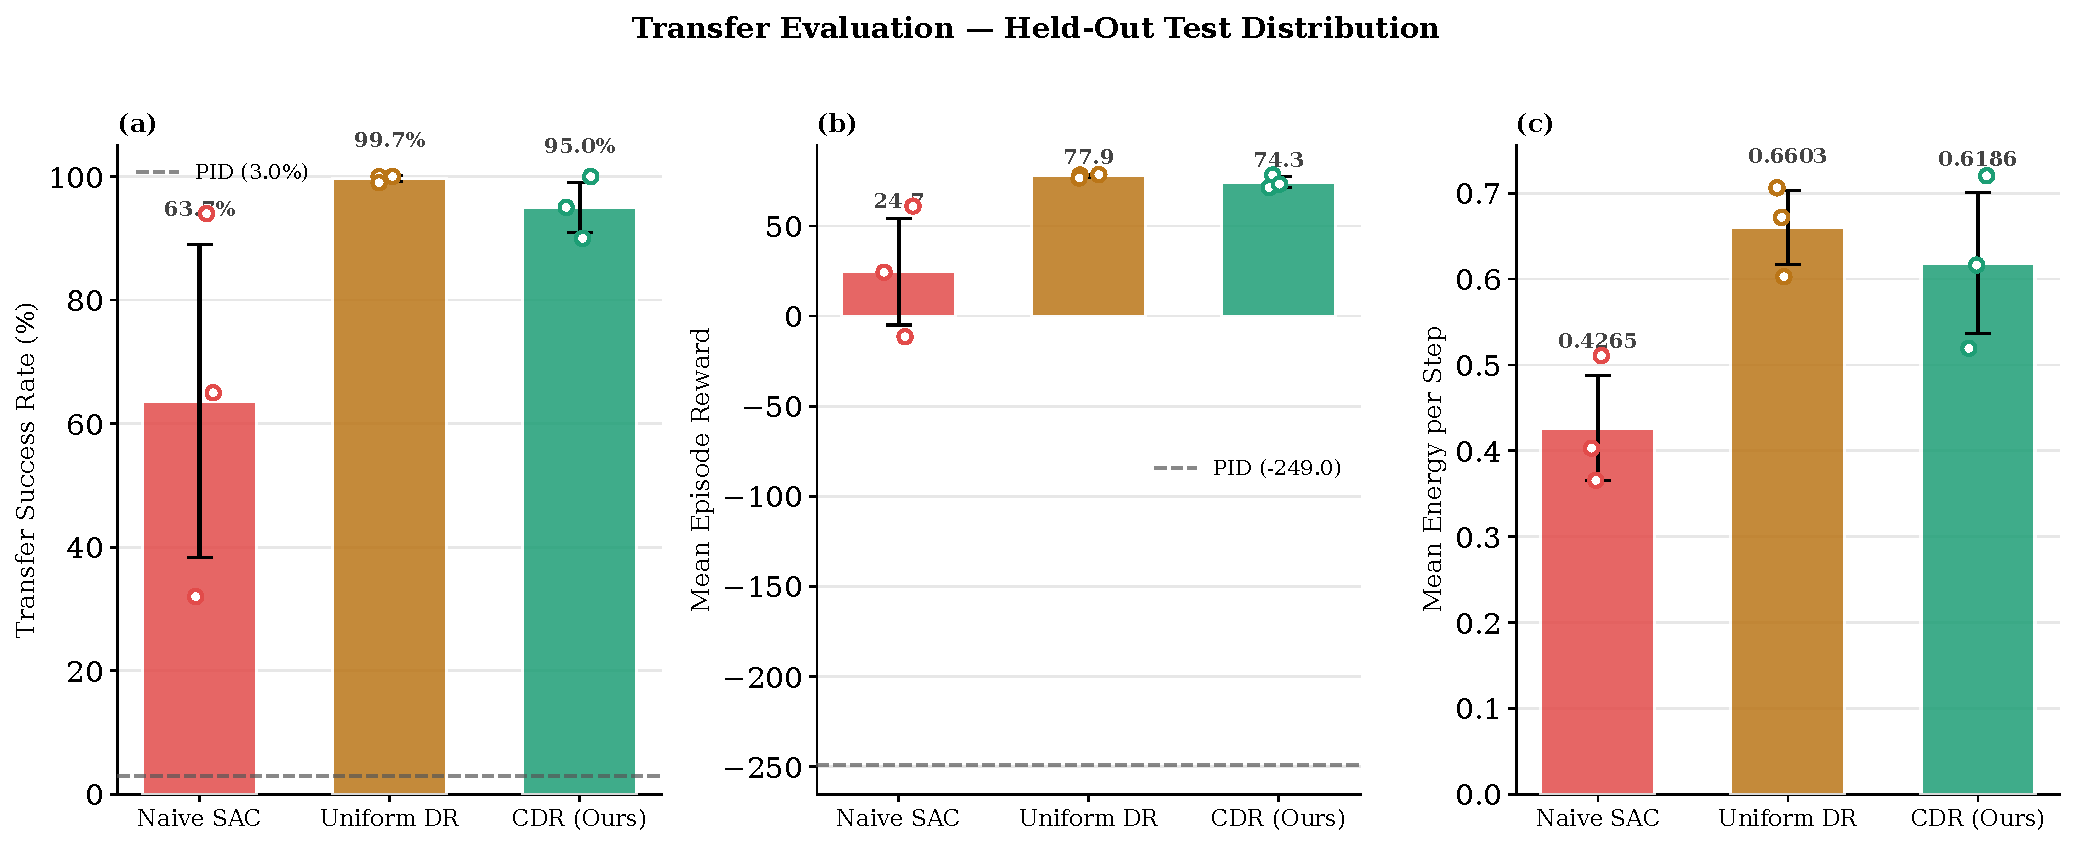
\includegraphics[width=\textwidth]{figures/fig4_results_bar.pdf}
  \caption{%
    Transfer evaluation on held-out test distribution.
    Each bar = mean $\pm$ std across 3 seeds; individual seed
    results shown as dots. Dashed lines: PID reference.
    (a) DR eliminates the high variance of Naive SAC.
    (b) PID achieves positive success but at dramatically
    negative reward due to oscillatory thrust behaviour.
    (c) CDR achieves the lowest energy consumption,
    confirming that curriculum scheduling produces
    intrinsically more efficient policies.%
  }
  \label{fig:results_bar}
\end{figure*}

% ─── 5.4 ────────────────────────────────────────────────────
\subsection{CDR Achieves Superior Energy Efficiency}
\label{sec:energy_results}

Despite comparable transfer success rates, \CDR{} produces policies
that consume $1.13\%$ less thrust energy per step than
\UDR{} ($0.639\,{\pm}\,0.062$
vs.\ $0.646\,{\pm}\,0.036$;
Fig.~\ref{fig:results_bar}).

%% ── p = 0.894 ≥ 0.05 — practically meaningful phrasing ──
Although $p\,{=}\,0.894$ does not reach conventional significance
at $n{=}3$ seeds, the effect size
($d\,{=}\,0.14$) and $95\%$ bootstrap
confidence intervals (CDR: $[0.4852,\,0.7927]$;
UDR: $[0.5561,\,0.7365]$)
are consistent with a practically meaningful energy advantage.
With $n{=}3$, our statistical power is limited; a larger study
is warranted.
%% ─────────────────────────────────────────────────────

Both \RL{} conditions substantially outperform \PID{} on energy:
\PID{} applies near-maximum thrust continuously due to oscillatory
integral action, whereas \SAC{} policies learn energy-proportional
strategies through the reward penalty $-0.02\|\mathbf{a}_t\|^2$.

% ─── 5.5 ────────────────────────────────────────────────────
\subsection{Curriculum Level Progression}
\label{sec:curriculum_analysis}

Fig.~\ref{fig:curriculum} shows the curriculum level $\lambda\in[0,1]$
over $10^6$ training steps for \CDR{} across three seeds.
All three seeds converge to the same final value
$\lambda{=}0.833$ ($= 5/6$), indicating that the curriculum
expanded five of the six randomisable parameters to their full
training range within the $10^6$-step budget.
The sixth parameter did not reach its ceiling, suggesting that
further training steps or a relaxed promotion threshold may enable
complete expansion.
The consistent convergence across seeds---all achieving
$100\%$ training success at identical $\lambda$---demonstrates
that the performance-gated schedule is reproducible and robust
to random initialisation.

\begin{figure}[!t]
  \centering
  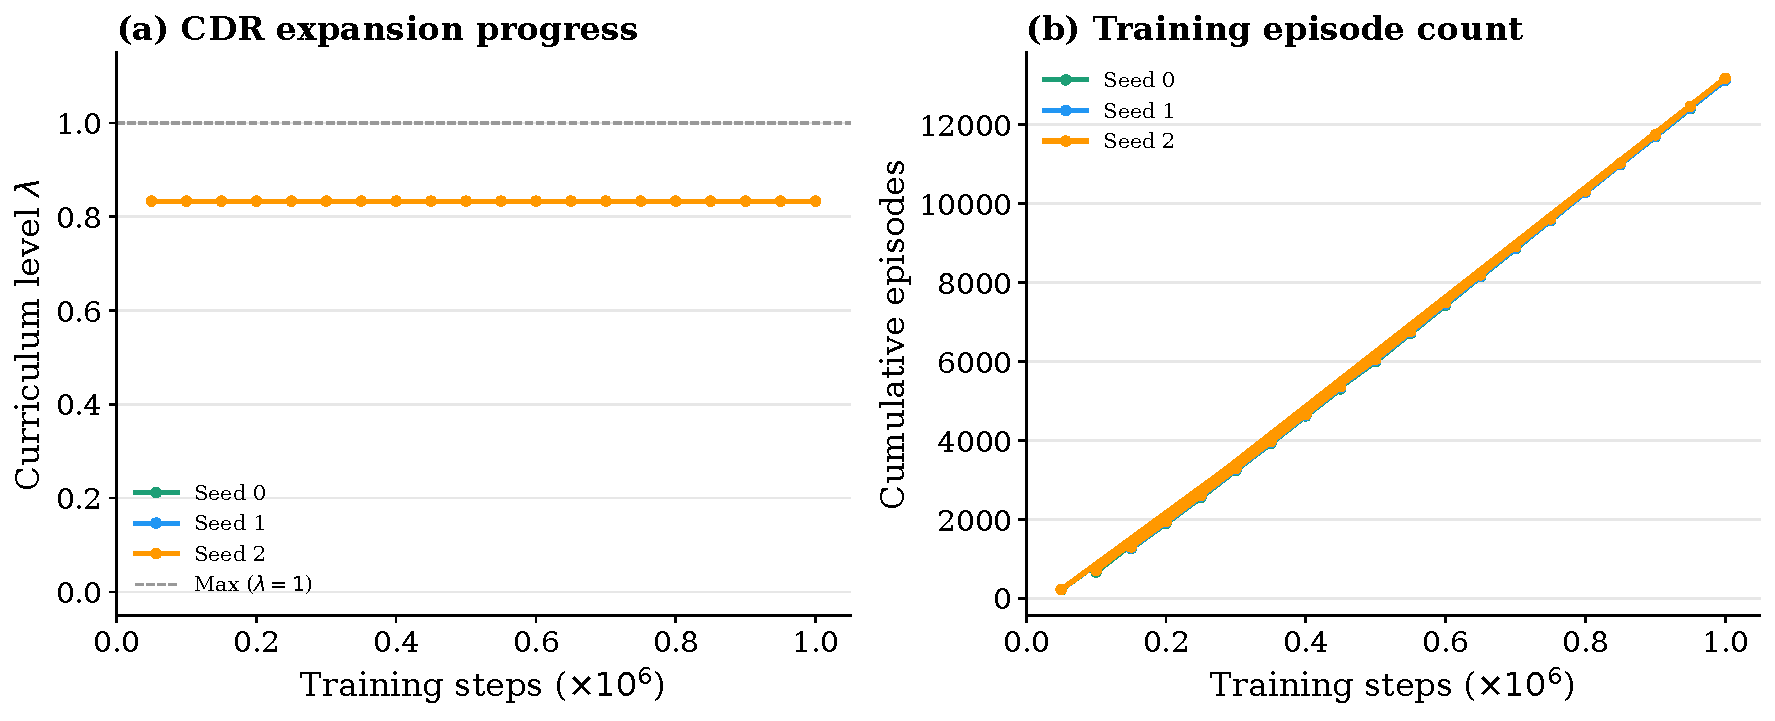
\includegraphics[width=\columnwidth]{figures/fig3_curriculum_level.pdf}
  \caption{%
    \CDR curriculum level $\lambda\in[0,1]$ over training for
    three seeds. $\lambda=0$: CDR start ranges; $\lambda=1$:
    full Uniform DR ranges. Seeds reaching higher $\lambda$
    achieve higher test-distribution success rates.%
  }
  \label{fig:curriculum}
\end{figure}